%%%%%%%%%%%%%%%%%%%%%%%%%%%%%%%%%%%%%%%%%%%%%%%%%%%%%%%%%%%%
%%
%% WIKIPEDIA
%%
%%%%%%%%%%%%%%%%%%%%%%%%%%%%%%%%%%%%%%%%%%%%%%%%%%%%%%%%%%%%
\section{Wikipedia}
\subsection*{In academia}
Wikipedia is a free, open-source, publicly-editable online
knowledge-base. The software is runs upon, PHP-based MediaWiki, is
also open-source, powering countless other online encyclopedias. The
website is ranked 6\super{th} globally in terms of website traffic,
and is the highest-ranked reference website by far - most of the sites
it shares the top spots with are portals, search engines, shopping
mega-sites, and social media websites.\footnote{According to `Alexa',
  an website ranking company.\cite{Alexa-about2014} Though, this may
  be an underestimation. Alexa may well be biased towards English
  speakers and Internet Explorer users, underestimating
  Wikipedia.org's popularity, since `two thirds of all Wikipedia
  articles are in languages other than
  English'\cite{wikimedia-noteonalexa}} Despite early skepticism
(particularly concern over the inherent chaos in the system:
``...edits, contributed in a predominantly undirected and haphazard
fashion by ... unvetted volunteers.''\cite{Wilkinson2007}), it is
widely claimed to be a success, `the best-developed attempt thus far
of the enduring quest to gather all human knowledge in one
place'\cite{Mesgari2014}.

That Wikipedia has become a hub of research in many fields is also
self-evident to anyone who has searched for articles on the
subject. Mesgari et al, just quoted, has prepared a very recent
`systematic review of scholarly research on the content of Wikipedia',
which gives an overview of 110 articles on the subject --- attesting
to his observation that Wikipedia has been `irresistable point of
unquiry for researchers from various fields of knowledge'. It will be
a useful touching stone for this study, finding 82 out of the 110
surveyed articles to concern Wikipedia quality. Some of these are also
referenced here, and many of the others will come to bear on the study
as it progresses.

Other important general sources will be WikiLit,\cite{wikilit}
AcaWiki\cite{acawiki} and WikiPapers\cite{wikipapers}, all of which
are online repositories of academic research into Wikipedia and other
Wikis.

%%%%%%%%%%%%%%%%%%%%%%%%%%%%%%%%%%%%%%%%%%%%%%%%%%%%%%%%%%%%
%%
%% WIKIPEDIA ARTICLE QUALITY
%%
%%%%%%%%%%%%%%%%%%%%%%%%%%%%%%%%%%%%%%%%%%%%%%%%%%%%%%%%%%%%

\subsection*{Studies of Wikipedia revision history}
Tangentialy related studies fall into two major groups: studies of
Wikipedia article quality and studies of edit behaviour.  It is from
the first group that we find the most pertinent work --- it is also
one of the most fruitful areas of research.

It is the metrics used to measure quality in these studies that are of
most use to us here. We don't concern ourselves with the quality of
the article on the whole, but many studies have endeavoured to find
out what kind of article content can be automatically recognised. High
numbers of Links, internal links, images and formulas have been found
to indicate percieved quality,\cite{Lucassen2010}\cite{mcguinness2006}
and these are easy to identify using Wikipedia's markup
language. Other useful meterics have been the age of the
word,\cite{Cross2006} the age and rate of change of the article in
comparison to other articles,\cite{Zeng2006} and the recent activity
of the article (an article undergoing a peak in edit changes may be
`unstable').\cite{Adler2006} Another study of particular interest is
that of Stvilia et al, which found metrics of article quality through
factor analysis,\cite{Stvilia2005} confirming much of the ideas
already mentioned.

A landmark piece of work is the Wikitrust software.\cite{Adler2007}
Wikitrust was\footnote{Defunct as of author's checks, Apr 2014} a
firefox plugin, designed to highlight the words of a Wikipedia article
with different colors. The gradations of these colors relate to levels
of trust, and the computations made to derive them were based upon the
metrics mentioned above, with particular emphasis on a word's age. A
screenshot can be seen in figure \ref{fig:wikitrust}. The program was
reviewed as recently as 2011,\cite{Lucassen2011} and it was found to
be basically flawed, with users not really seeing the use for it (it
was found that, having read Wikipedia before, they already had a good
idea of how to rate an article). However, the Wikitrust team's
implementation of the quality measures described above will prove to
be very useful study.

\begin{figure}
  \centering
  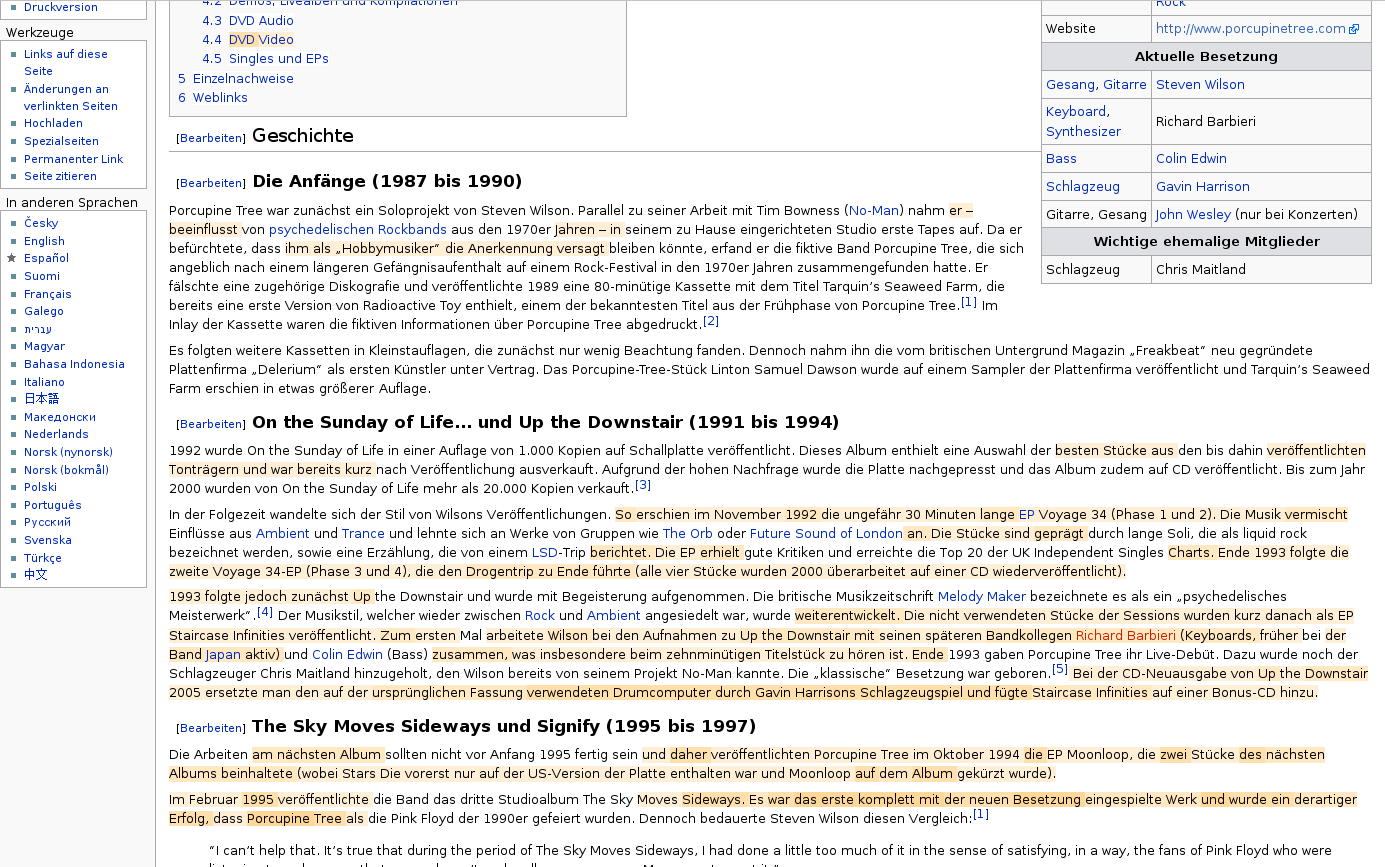
\includegraphics[width=0.8\textwidth,clip=true,resolution=300]{img/wikitrust.png}
  \caption{Wikitrust in action, 2011}
  \label{fig:wikitrust}
\end{figure}

Another metric which may also affect the quality of an article as a
resource, is logical structure. It was found in 2005 that this, if
anything, was the clearest difference between Wikipedia and commercial
encyclopedias,\cite{Giles2005} supporting previous
conjecture.\cite{Denning2005} Not many studies have concerned
themselves with structure, but later we will discuss how we may
automatically recognise structural change.

A few other key studies present us with useful analyses of edit
behaviour. Analyses of conflict between authors shows the possible
reversion cases we will have to recognise. They reveal the high number
of immediate `undo'-type revisions, and also that malicious or
unnecessary input may survive several versions before being
undone. Some study these conflicts as a characterisation of normal
editing
behaviour,\cite{Kittur2007}\cite{Kittur2009}\cite{Kittur2010}\cite{Potthast2008}
while others look to controversial articles,\cite{Iba2010} or articles
recently cited in the press.\cite{Lih2004} We find from these same
studies that articles lead by small groups of `leaders' produce
articles of better quality than those with a more homogeneous
contribution group, that a small group of editors contribute to most
of Wikipedia, and that conflict and bureaucracy (increasing over time)
are the major limiting factors in the growth of an
article.\cite{Suh2009} Knowledge of this context is vital in
evaluating the edits we will eventually analyse.
